\documentclass[a4paper,11pt]{article}
\usepackage{graphicx}
\usepackage{url}
\usepackage{hyperref}
\usepackage{amsmath}
\usepackage{listings}
\begin{document}

\title{Recurrent Neural Networks for Predicting Bitcoin prices\\
\normalsize (MP 100 VietNguyen)}

\author{Viet Nguyen Tuan (533302)}

\maketitle

\newcommand{\points}[1]{\par\noindent\textit{(#1 points)}}
\newcommand{\onepoint}{\par\noindent\textit{(1 point)}}



\begin{abstract}
 
  This projects aims at predicting cryptocurrencies price using deep learning methods, particularly recurrent neural networks. The performance of both approaches has been boosted by
  preprocessing the datasets, including data normalization. Experiments including various parameter settings has also been carried out to select the best possible parameters
  %% 
  \onepoint
\end{abstract}

\section{Introduction}

%Describe the machine learning problem you have addressed in your mini
%project, your applied method and used data in general terms.
%%

\points{2}



The goal of this project is to build a model that can successfully predict the cryptocurrency price in the short-term future. The data is taken from blockchain.info using code from Kaggle dataset  \href{https://www.kaggle.com/sudalairajkumar/cryptocurrencypricehistory/data}{Cryptocurrency Historical Prices}
Recurrent neural network using Bidirectional LSTM layers has been fit to the data multiple time with multiple settings in order to select the best performing model



\section{Related work}

%Give a brief literature survey on the prior works and state of the art
%in the problem setting and the methods people have earlier applied for
%solving it.

%%
\points{2}

\noindent There are many prior works on this topic which could be viewed from Kaggle \href{https://www.kaggle.com/sudalairajkumar/cryptocurrencypricehistory/kernels}{Cryptocurrency Historical Prices}. Most of the previous kernel use regression analysis and other basic time series forecasting model like exponential smoothing to build the predictive model. I, however, decide to use deep learning approach to see if this is perform better than the others	

\section{Method}

%Describe your chosen solution in sufficient detail.  Pay special
%attention to describing the deep learning algorithm(s) you used.  Show
%some essential equations and describe all hyperparameters that are
%involved in the method.
%%
\points{3}
\noindent Our study relies on the assumption that the price of the cryptocurrency follows some particular patterns that based on past historical data. Therefore we think RNNs maybe good at this task.

\noindent Recurrent neural network (RNN) is a neural network with self-loop in its hidden layer(s), which enables RNN to use the previous state of the hidden neuron(s) to learn the current state given the new input. RNN is good at processing sequential data. The problem with normal RNNs is that they are unable to learn long-term dependencies, i.e., connect the previous information to current task


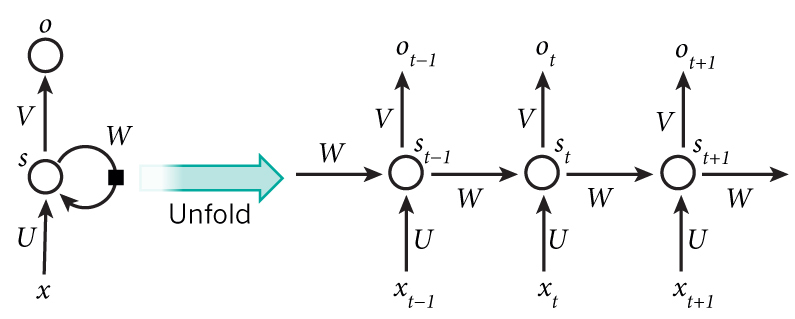
\includegraphics[height = 5cm]{figure1.jpg}

\noindent Long Short Term Memory networks (LSTMs) are a variant of RNN, which can fully address the problem of learning long-term dependencies that RNNs have. Like RNNs, LSTM also has chain-like structure, but with four layers (instead of one) interacting in a very special way.


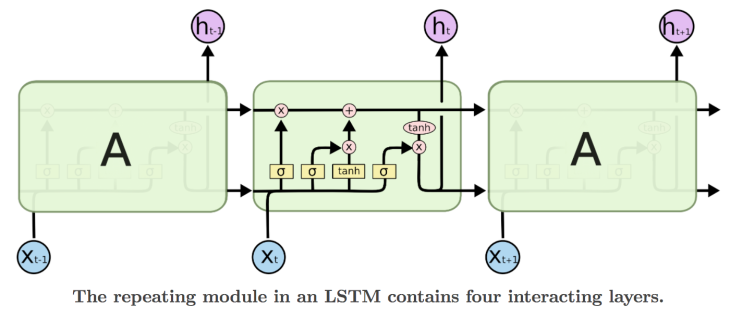
\includegraphics[height = 5cm]{figure2.png}

From the figure, we can see that the cell state run along the entire chain, depict by the horizontal line. Information can be removed or added to the cell state, through structures call gates

The LSTM does have the ability to remove or add information to the cell state, carefully regulated by structures called gates. In this model LSTM has three gates. Gates are made of a sigmoid neural net layer and computed by a pointwise multiplication operation. The sigmoid layers output (between 0 - 1) indicates how much of each information should be go through

There are 3 stages when information flows through the gates. The first step is the “forget gate layer” - this determines what information would be excluded from the cell state

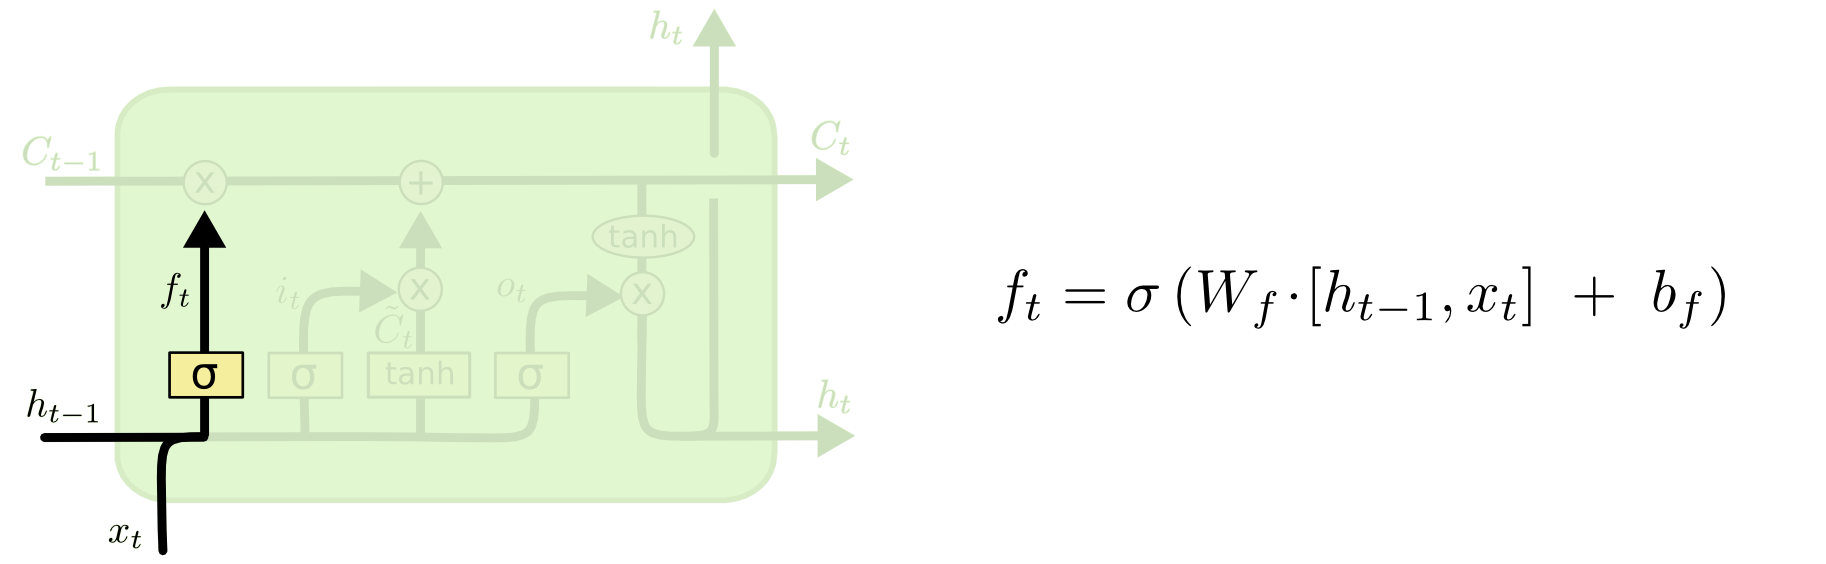
\includegraphics[height = 5cm]{ltsm1.png}

In the next step there are two layers determining what new information will be stored in the cell state. The sigmoid layer or the “input gate layer” select the values to update. After that, a new value vector $\tilde{C}_t$ are created by the "tanh" layer to add to the next stage. 

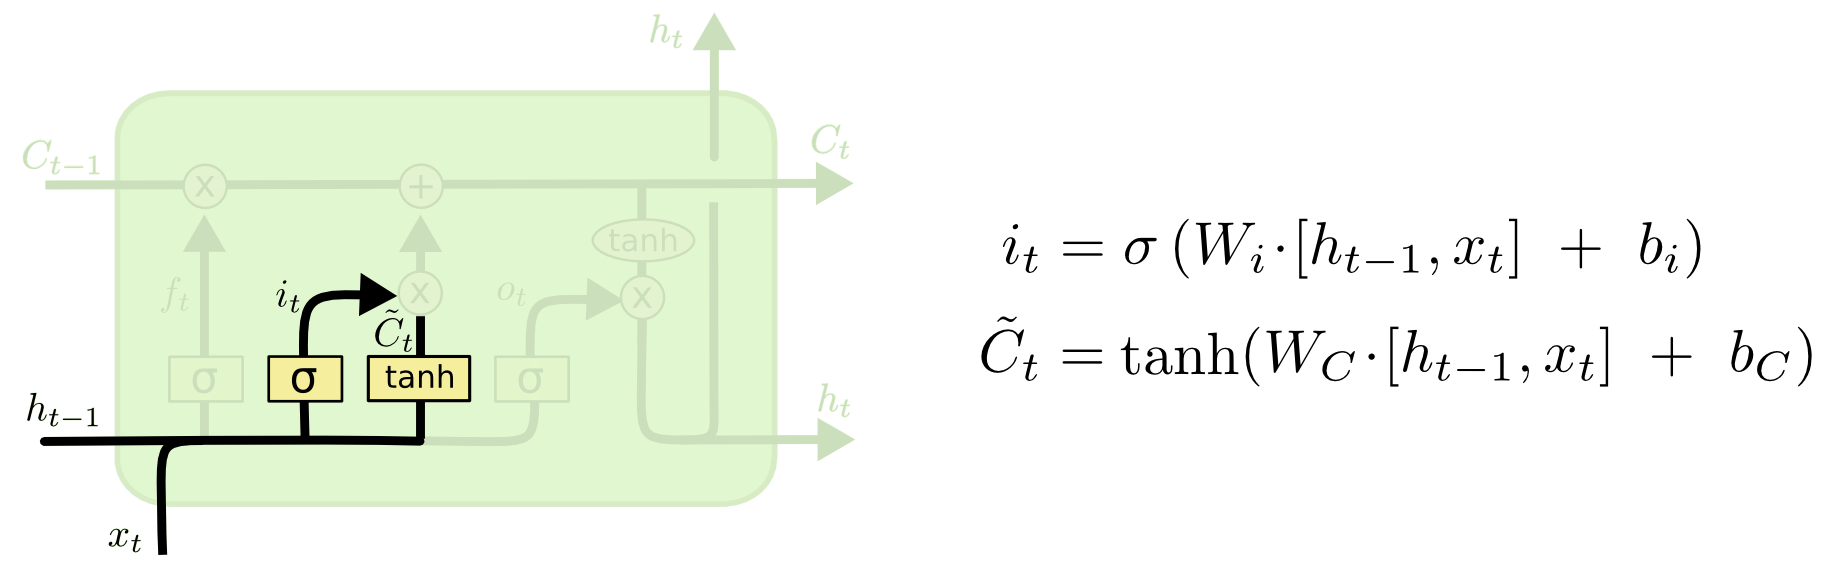
\includegraphics[height = 5cm]{ltsm2.png}


The next stage is to combine the result we get from previous two as follow:

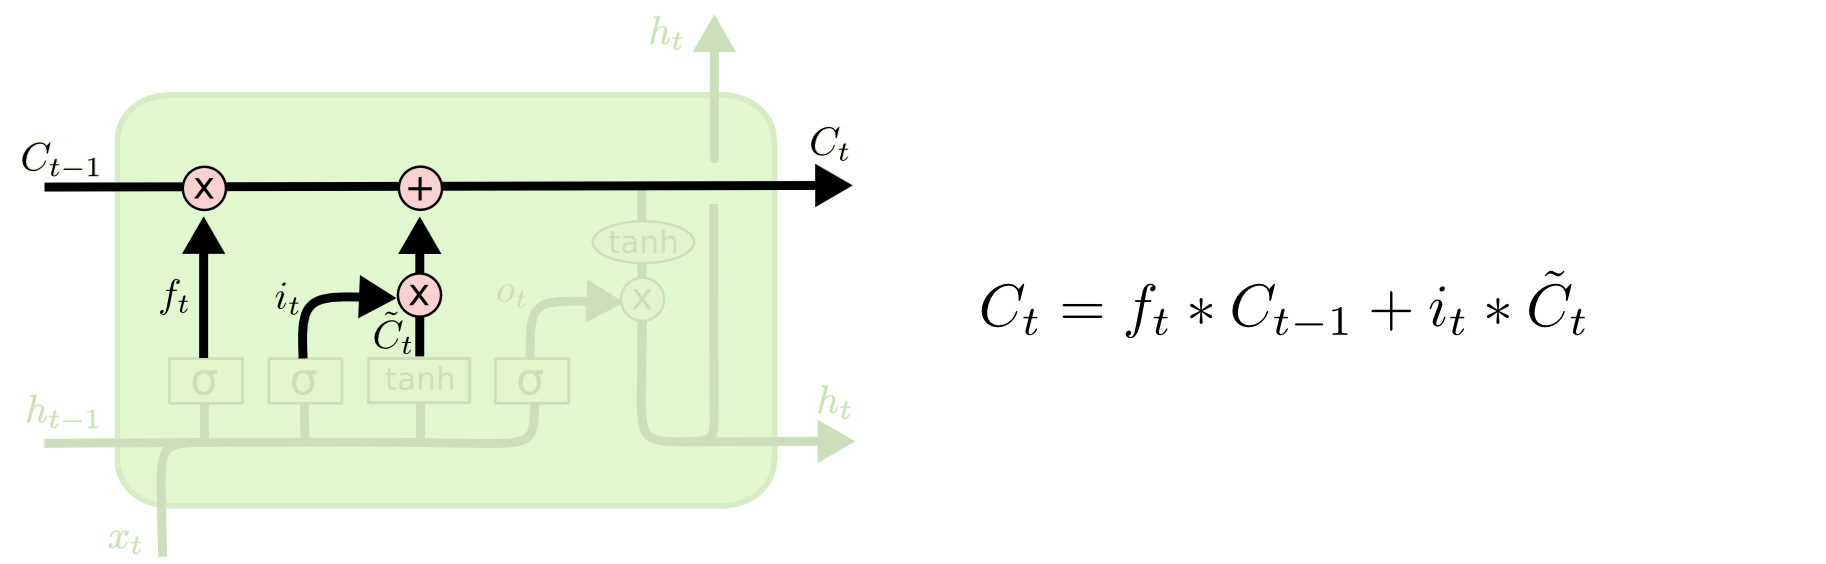
\includegraphics[height = 5cm]{ltsm3.png}

Finally,a sigmoid layer will be computed on the cell state, then the results are put through a "tanh" function in order to get the final output 

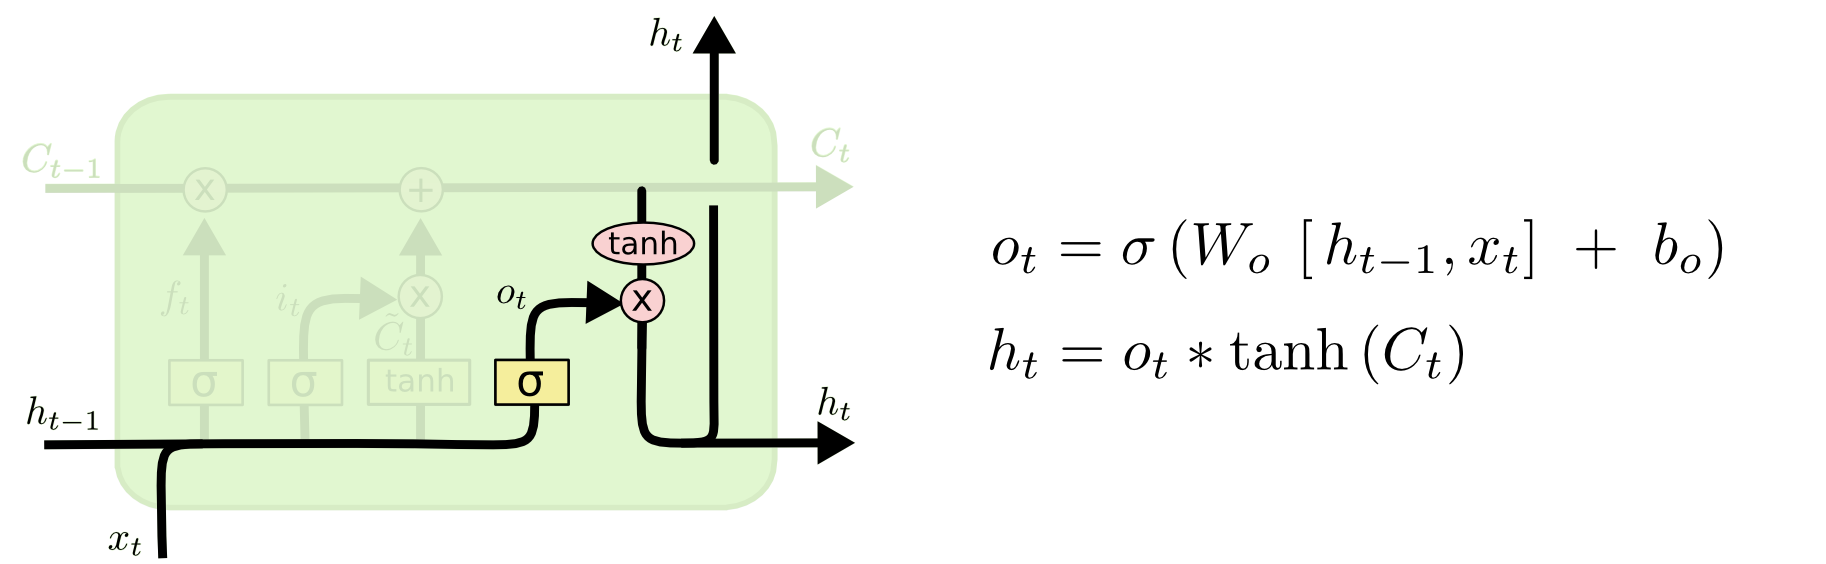
\includegraphics[height = 5cm]{ltsm4.png}

\noindent In this study we also decide to combine the LSTM with Bidirectional RNNs in order to increase the availability of information to the network. Bidirectional RNNs consists of two RNNs stacked on top of each other. The output is then computed based on the hidden state of both RNNs.


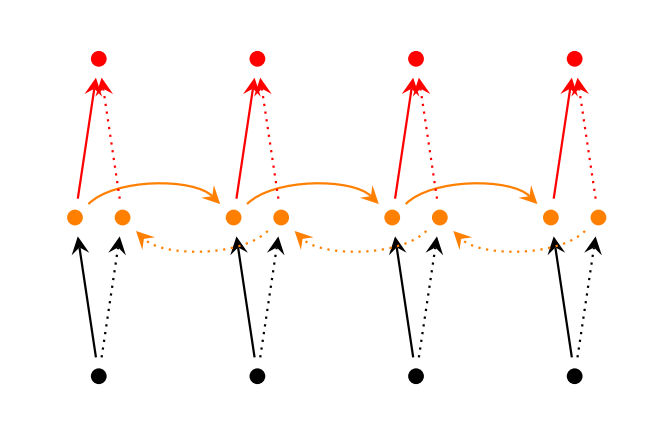
\includegraphics[height = 5cm]{figure3.png}

\section{Data}

%Tell where the data is from, what it contains, the number of samples
%in training, validation and test sets, the dimensional, etc.  Also
%describe the preprocessing stages applied by the providers of the data
%or by you yourselves.
%%
\points{3}

The data is obtain from blockchain.info, which includes 23 features regarding the bitcoin (the cryptocurrency chosen in this study). Here is the link of the data. The features are quite explanatory from the urls

\begin{lstlisting}
'https://blockchain.info/charts/market-price',
'https://blockchain.info/charts/total-bitcoins',
'https://blockchain.info/charts/market-cap',
'https://blockchain.info/charts/trade-volume',
'https://blockchain.info/charts/blocks-size',
'https://blockchain.info/charts/avg-block-size',
'https://blockchain.info/charts/n-orphaned-blocks',
'https://blockchain.info/charts/n-transactions-per-block',
'https://blockchain.info/charts/median-confirmation-time',
'https://blockchain.info/charts/hash-rate',
'https://blockchain.info/charts/difficulty',
'https://blockchain.info/charts/miners-revenue',
'https://blockchain.info/charts/transaction-fees',
'https://blockchain.info/charts/cost-per-transaction-percent',
'https://blockchain.info/charts/cost-per-transaction',
'https://blockchain.info/charts/n-unique-addresses',
'https://blockchain.info/charts/n-transactions',
'https://blockchain.info/charts/n-transactions-total',
'https://blockchain.info/charts/n-transactions-excluding-popular',
'https://blockchain.info/charts/n-transactions-excluding-chains
-longer-than-100',
'https://blockchain.info/charts/output-volume',
'https://blockchain.info/charts/estimated-transaction-volume',
'https://blockchain.info/charts/estimated-transaction-volume-usd'
\end{lstlisting}

The data is transformed from \textit{(num days x num features)} to \textit{(num days- window size x num days per sample x num features)} with the window size of 49. 

To be clear, the original data with shape (2920, 23) has been processed into training data of (2583, 49, 23) and testing data of (287, 49, 23) with 49 is the window size

Zeros and NaNs values are replaced with the value before they appear. 

Then the data is normalized in which each value in the window is divided by the first value in the window and then subtracting one i.e [4,3,2] into [0, -0.25, -0.5]

The training set comprises of 90\% of the data while the rest 10\% is used in the test set



\section{Experiments}

%Explain the goal and implementation of your experiments.  Tell what
%hyperparameters values you experimented with and what other
%variations in the method you tested.
%%
\points{5}

Implementation of LSTM and bidirectional RNNs in this study is done using Keras. Sequential() model is used with 3 recurrent layers, the first 2 layers has a dropout value that representing how much information are dropped at each level. The window size represents how many days of training values that the model can look at once.

Other parameters of the models:
\begin{lstlisting}
 
batch_num : (int) batch size (1024)
num_epoch : (int) number of epochs (100)
dropout_value : (decimal) representing how much dropout (0.2)
activation_function : the activation_function (linear)
loss_function : the loss function to be used (mean squared error)
optimizer : the optimizer to be used (adam)
\end{lstlisting}

Source code for the model:
\begin{lstlisting}
def initialize_model(window_size, dropout_value, 
	activation_function, loss_function, optimizer):
	model = Sequential()
	model.add(Bidirectional(LSTM(window_size), 
	input_shape=(window_size, X_train.shape[-1]),))
	model.add(Dropout(dropout_value))
	model.add(Bidirectional(LSTM((window_size*2))))
	model.add(Dropout(dropout_value))
	model.add(Bidirectional(LSTM(window_size)))
	model.add(Dense(units=1))
	model.add(Activation(activation_function))
	model.compile(loss=loss_function, optimizer=optimizer)
	return model
\end{lstlisting}

\section{Results}

%Give the results of your experiments in a table and explain them in
%the text.  Some figures would be good here for illustration.  Refer to
%the table(s) and image(s) in the text and describe them.
%%
\points{5}
Parameters settings for the experiment:
\begin{lstlisting}
dropout_value = 0.2
activation_function = 'linear
loss_function = 'mse'
optimizer = 'adam'
batch_num = 1024
num_epoch = 100
val_split = 0.5
\end{lstlisting}

Results of the experiment:

Comparison of predicted vs test price:

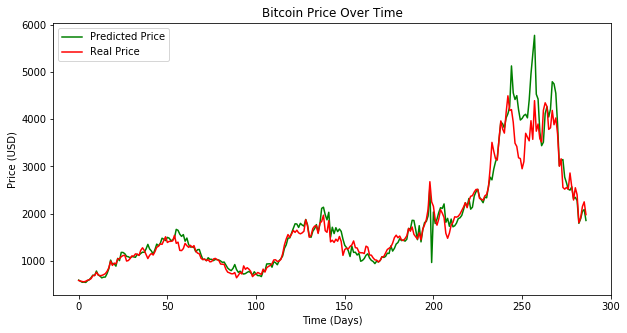
\includegraphics[height = 5cm]{ex1.png}

Comparison of predicted percent change vs test percent change:

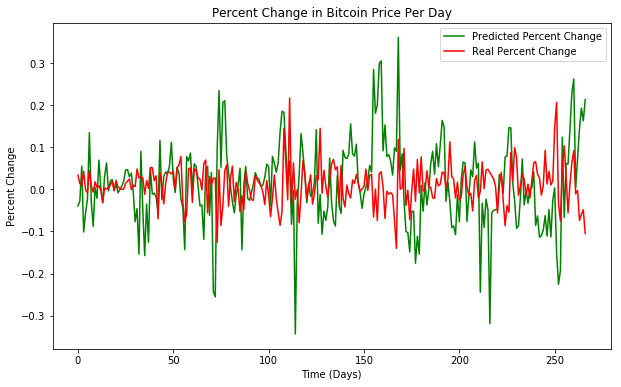
\includegraphics[height = 5cm]{ex1_2.png}

Other statistics:
\begin{lstlisting}
True positives: 93
False positives: 57
True negatives: 42
False negatives: 75

Precision: 0.62
Recall: 0.553571428571
F1 score: 0.584905660377
Mean Squared Error: 0.0430756924477
0.584905660377
\end{lstlisting}

\section{Discussion}

%Discuss your results in comparison with comparable results your have
%found in the literature and web.  Explain any other findings you made
%while running the experiments.
%%
\points{4}

We can see that our models give quite a decent result on predicted price, but not so satisfactory result on the percent change.
Take a quick look with results from the web, particularly   \href{https://www.kaggle.com/ara0303/forecasting-of-bitcoin-prices}{this one}
(using bayesian regression) and \href{https://www.kaggle.com/adamaulia/bitcoin-forecasting-using-mlp-sklearn}{this one}  (using multilayer perceptron), the performance are more or less the same compared to our model (although on old dataset)
\section{Conclusions}

%Give your final conclusions from the whole mini project and its results.
%%
\points{3}

With precision of 0.62, LSTM and bidirectional RNNs give a decent result on predicting the cryptocurrency prices. However, in order to make profit in the market, we need to fine-tune our model and increase its performance

\section{References}

%Most likely between 5--10 references to related works and results.
%%
\points{2}


Felix A. Gers; Jürgen Schmidhuber; Fred Cummins (2000). "Learning to Forget: Continual Prediction with LSTM". Neural Computation. 


Schuster, Mike, and Kuldip K. Paliwal. "Bidirectional recurrent neural networks." Signal Processing, IEEE Transactions on 45.11 (1997)


\href{https://arxiv.org/pdf/1705.05690.pdf}{A Long Short-Term Memory Recurrent Neural Network Framework for Network Traffic Matrix Prediction}


Keras documentation

\end{document}